\section{Datos de entrada}
\label{ch:implementacion:sec:datosDeEntrada}

\subsection{Requerimientos}
\label{ch:implementacion:sec:datosDeEntrada:subsec:requerimientos}

Para poder utilizar el algoritmo de \emph{MarchingCubes}, se necesita que cada punto de un espacio tridimensional tenga asociado un valor dentro de un rango definido de manera que cada punto pueda describirse como un vector de cuatro dimensiones compuestas por sus coordenadas y un valor escalar, como muestra el vector \ref{ch:implementacion:sec:datosDeEntrada:vector}.

\begin{equation}
\label{ch:implementacion:sec:datosDeEntrada:vector}
	(x,y,z,v)
\end{equation}

Por ejemplo, en una habitación se tiene un foco de luz en el centro emitiendo luz en todas direcciones, con esto, cada punto de la habitación percibe distintas instensidades de luz que depende de la distancia al foco, mientras mas cerca del foco, mayor intensidad, mientras mas alejado del foco, menor intensidad. Si de alguna manera pudiesen marcase todos aquellos puntos que tengan una intensidad específica, se tendría una esfera formada por puntos equidistantes al foco, ya que todos ellos comparten la misma intensidad, por lo que se dice que esa es la superficie que encierra a todos los puntos con una cierta intensidad o mayor.

Ciertamente, el algoritmo también sirve para visualizar gráficos en tres dimensiones, usando el mismo principio, cada punto del espacio tiene un valor asociado el cual es calculado por la ecuación. Para poder dibujar la susperficie se puede transformar la ecuación en una inecuación y luego marcar todos aquellos puntos que sean menores que el valor entregado por la ecuación, por ejemplo se tiene en la ecuación \ref{ch:implementacion:sec:datosDeEntrada:ec1}:

\begin{equation}
\label{ch:implementacion:sec:datosDeEntrada:ec1}
	x^{2} + y^{2} = 1
\end{equation}

Para poder graficar esta ecuación usando \emph{MarchingCubes} se debe transformar la ecuación en una inecuación como se muestra en la ecuación \ref{ch:implementacion:sec:datosDeEntrada:ec2}:

\begin{equation}
\label{ch:implementacion:sec:datosDeEntrada:ec2}
	x^{2} + y^{2} <= 1
\end{equation}

Dependiendo de la resolución escogida, es posible que algunos cubos tengan algunos de sus vértices con coordenadas $(x,y)$ que satisfacen a la inecuación, por lo tanto quedan marcados como vértices internos, luego el proceso es ir iterando en todos esos cubos y reemplazando los cubos por los triángulos que correspondan a los quince casos mostrados en la figura \ref{f:estadoDelArte:Shu95adaptivemarching_1}.

\subsection{Datos como cortes de nivel}
\label{ch:implementacion:sec:datosDeEntrada:subsec:datoscomocurvasdenivel}

Otra forma de entregar datos de entrada es teniendo cortes de nivel de un cuerpo tridimensional, un ejemplo de esto son las imágenes obtenidas de los exámenes de resonancia magnética. Cada imagen representa un corte transversal del cuerpo estudiado, como el que se mostró en la figura \ref{f:flujoDeTrabajo:mri_joe}.

Éstas imágenes, en conjunto, describen un cuerpo en tres dimensiones, mostrando con detalle sus componentes internos. Cada imágen está compuesta por una matriz de pixeles en una escala de grises, dependiendo de la profundidad de color, pueden ser de 256 valores (8 bits) o de 65536 valores (16 bits) diferentes, con estas imágenes se puede construir un espacio que puede servir como entrada para el algoritmo de \emph{MarchingCubes}, una forma de hacerlo es usando las coordenadas en 2 dimensiones del pixel en una imagen y usando como valor $z$, el número que representa la imagen dentro del cuerpo. Una vez identificado el pixel en un espacio tridimensional, el valor de éste pixel está determinado por la intensidad de color del pixel, como se muestra en el vector \ref{ch:implementacion:sec:datosDeEntrada:ec3}:

\begin{equation}
\label{ch:implementacion:sec:datosDeEntrada:ec3}
	(x,y,z,color)
\end{equation}

Para ejemplificar, considere dos imágenes de $2x2$ pixeles, esto crea 8 pixeles en total, suficientes para que cada pixel represente un vértice de un cubo, luego cada pixel determina el valor del vértice usando la tonalidad gris del pixel asociado. En la figura \ref{f:implementacion:images_minimal}, se muestra éste caso, usando 2 imágenes cuyos pixeles tienen una tonalidad de gris de 97, en una escala de 0 a 255 (8 bits), excepto el pixel (0,0) de la primera imagen (imagen \#0).

\begin{figure}[!hbt]
	\centering
	
\includegraphics[width=0.6\textwidth]{images/misc/images_minimal.pdf}
	\caption{Dos imágenes de $2x2$ pixeles cada una, cada pixel está etiquetado con su respectivo vector de 4 dimensiones.}
	\label{f:implementacion:images_minimal}
\end{figure}

Si se aplica \emph{Marching Cubes} en este caso usando un valor mínimo de $100$, casi todos los vértices cumplirían la condición ya que casi todos los vértices tienen un valor de $97$, excepto el vértice correspondiente al pixel $(0,0,0)$ (primer pixel de la imagen \#0), por esto, es el único vértice no marcado, quedando así un cubo que solo necesita de un sólo triángulo que separa a este vértice de los demás, como se muestra en la figura \ref{f:implementacion:images_minimal_cube}.

\begin{figure}[!hbt]
	\centering
	
\includegraphics[width=0.3\textwidth]{images/misc/images_minimal_cube.pdf}
	\caption{El resultado de aplicar \emph{Marching Cubes}, solo se obtiene un triángulo que separa al vertice blanco, de los demás.}
	\label{f:implementacion:images_minimal_cube}
\end{figure}

En esta implementación, se usó este último método para obtener una nube de puntos para poder extraer una superficie utilizando \emph{Marching Cubes}.

%TODO: poner link al glosario, en 'dataset'
Las imágenes de la figura \ref{f:implementacion:dataset:ImSphRad100} muestran algunas de las imágenes de un \emph{dataset} que describe una esfera mediante cortes transversales.

\begin{figure}
\centering

	\begin{subfigure}{0.30\textwidth}
		\centering
		
\includegraphics[width=\textwidth]{images/datasets/ImSphRad100/Sphere001.png}
		\caption{Imagen \#001}
		\label{f:implementacion:ImSphRad100:001}
	\end{subfigure}
	%~
	\begin{subfigure}{0.30\textwidth}
		\centering
		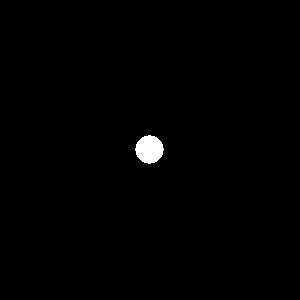
\includegraphics[width=\textwidth]{images/datasets/ImSphRad100/Sphere051.png}
		\caption{Imagen \#051}
		\label{f:implementacion:ImSphRad100:051}
	\end{subfigure}
	%~
	\begin{subfigure}{0.30\textwidth}
		\centering
		
\includegraphics[width=\textwidth]{images/datasets/ImSphRad100/Sphere070.png}
		\caption{Imagen \#070}
		\label{f:implementacion:ImSphRad100:070}
	\end{subfigure}

	\begin{subfigure}{0.30\textwidth}
		\centering
		
\includegraphics[width=\textwidth]{images/datasets/ImSphRad100/Sphere102.png}
		\caption{Imagen \#102}
		\label{f:implementacion:ImSphRad100:102}
	\end{subfigure}
	%~
	\begin{subfigure}{0.30\textwidth}
		\centering
		
\includegraphics[width=\textwidth]{images/datasets/ImSphRad100/Sphere166.png}
		\caption{Imagen \#166}
		\label{f:implementacion:ImSphRad100:166}
	\end{subfigure}
	%~
	\begin{subfigure}{0.30\textwidth}
		\centering
		
\includegraphics[width=\textwidth]{images/datasets/ImSphRad100/Sphere218.png}
		\caption{Imagen \#218}
		\label{f:implementacion:ImSphRad100:218}
	\end{subfigure}

	\begin{subfigure}{0.30\textwidth}
		\centering
		
\includegraphics[width=\textwidth]{images/datasets/ImSphRad100/Sphere241.png}
		\caption{Imagen \#241}
		\label{f:implementacion:ImSphRad100:241}
	\end{subfigure}
	%~
	\begin{subfigure}{0.30\textwidth}
		\centering
		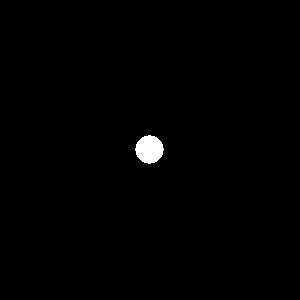
\includegraphics[width=\textwidth]{images/datasets/ImSphRad100/Sphere249.png}
		\caption{Imagen \#249}
		\label{f:implementacion:ImSphRad100:249}
	\end{subfigure}
	%~
	\begin{subfigure}{0.30\textwidth}
		\centering
		
\includegraphics[width=\textwidth]{images/datasets/ImSphRad100/Sphere300.png}
		\caption{Imagen \#300}
		\label{f:implementacion:ImSphRad100:300}
	\end{subfigure}

	\caption{Imágenes que describen una esfera}
	\label{f:implementacion:dataset:ImSphRad100}
\end{figure}

Éste dataset consta de 300 imágenes de $300 x 300$ pixeles con una profundidad de grises de 8 bits. Como se puede observar en la imagen \ref{f:implementacion:ImSphRad100:001} todos sus pixeles son negros, y considerando una profundidad de grises de 8 bits, es que todos sus pixeles valen $0$ (cero), sin embargo, la imagen \label{f:implementacion:ImSphRad100:051} muestra un pequeño círculo en su centro, por lo que aquellos pixeles que estan dentro del círculo, tienen un valor de $FF_{16} = 00_{2}$. A medida que nos acercamos a la imagen número 300, este cŕculo va creciendo hasta alcanzar un radio máximo, luego, su radio comienza a disminuir, hasta volver a un valor de cero. Describiendo de esta manera una esfera, en un espacio discreto de puntos de tamaño $300 x 300 x 300$

Ya que cada pixel, tiene asociado un par de coordenadas en 2 dimensiones, un número de imágen, y además un valor para especificar una tonalidad de gris, se puede describir cada pixel, como un vector de 4 dimensiones como se explicó en la seccion \ref{ch:implementacion:sec:datosDeEntrada:subsec:requerimientos}. Satisfaciendo los requerimientos que necesitan los datos de entrada para poder usar \emph{Marching Cubes}.

El resultado de aplicar \emph{Marching Cubes} a este \emph{dataset} se muestra en la figura \ref{f:implementacion:ImSphRad100:screenshot_40}, se puede apreciar como la esfera está formada por cortes transversales, cada uno describe un circulo cuyo radio va en aumento, y a medida que se acerca al final, disminuye. Además, se puede ver el efecto de escalonamiento (\emph{aliasing}) que presenta la superficie debido al uso de \emph{Marching Cubes}.

\begin{figure}[hbt]
	\centering
		\fbox
		{
			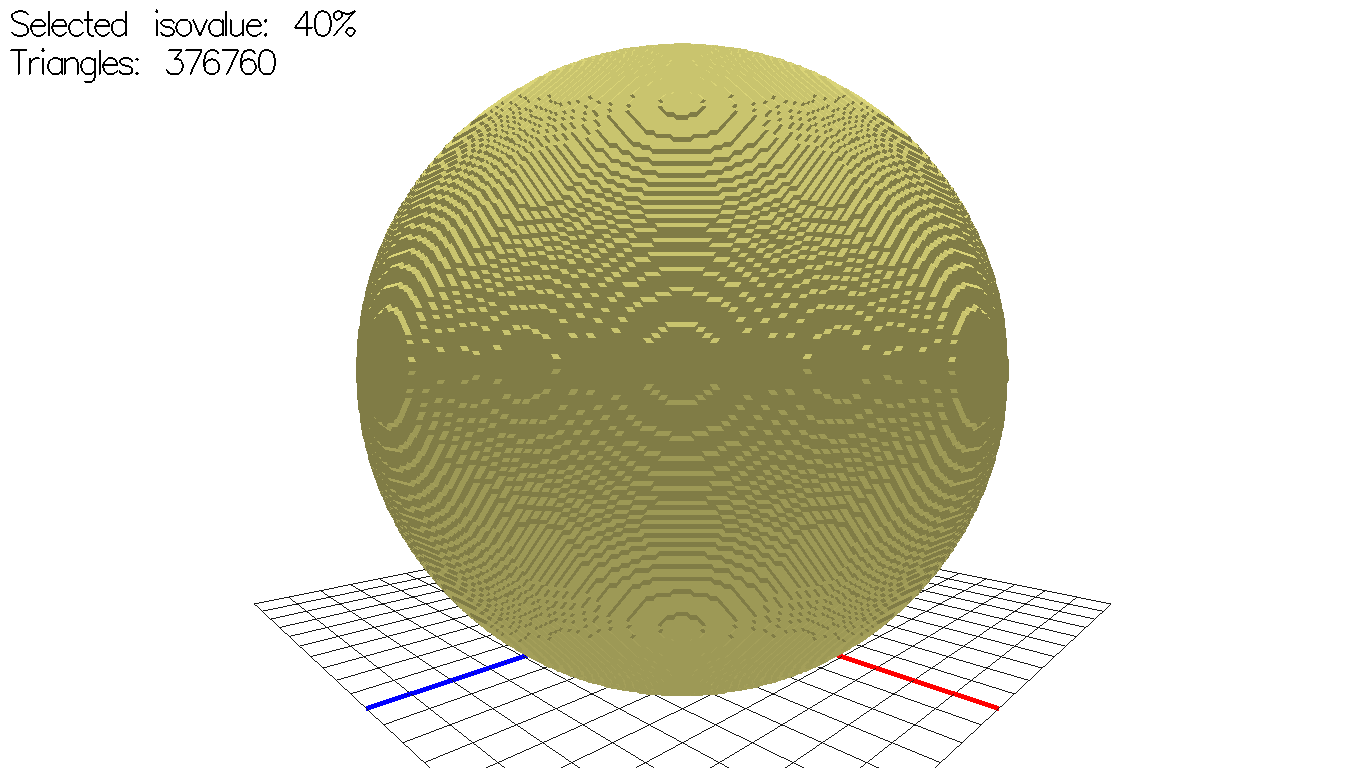
\includegraphics[width=0.95\textwidth]
			{images/results/ImSphRad100/screenshot_40.png}
		}
	\caption{La superficie extraida usando \emph{Marching Cubes} sobre un dataset que describe una esfera.}
	\label{f:implementacion:ImSphRad100:screenshot_40}
\end{figure}

\subsection{Formato de las imágenes de entrada}
\label{ch:implementacion:sec:datosDeEntrada:subsec:formatodelasimagenesdeentrada}

Idealmente, las imágenes utilizadas deberían estar todas en el mismo formato y compresión para ser utilizadas, también con la misma profundidad de colores (8 o 16 bits), pero esto no siempre es así.

%TODO: poner referencias a los formatos de imagenes, como svg y eso
Debido a que las imágenes provienen de orígenes y propósitos distintos, son obtenidas por distintos métodos, por ejemplo, uno puede crear imágenes de curvas de nivel de una ecuación tridimensional y con ellas generar un \emph{dataset} de imágenes en algún formato vectorial como SVG.

En el campo de la imagenología se usa el formato DICOM para la distribución digital de imágenes médicas, en las cuales, dentro de las imágenes hay información del paciente y otros datos relacionados con el estudio. De la misma manera, para efectos de investigación y publicación, se pueden encontrar en internet algunos \emph{datasets} que vienen en formato RAW, es decir, sin compresión alguna, y sin información alguna, sólo un arreglo de bytes los cuales representan un pixel de 8 bits continuados. Para poder leer estos archivos es necesario conocer anticipadamente las dimensiones tridimensionales del \emph{dataset}.

El algoritmo de \emph{Marching Cubes} es indiferente de cómo se obtengan los datos de entrada, mientras éstos puedan ser expresados como una nube de puntos tridimensionales, cada uno con un valor asociado dentro de un rango definido, como se explicó en la sección \ref{ch:implementacion:sec:datosDeEntrada:subsec:requerimientos}, por lo que para usar un \emph{dataset} de imágenes, la implementación debe poder extraer esta nube de puntos y valores asociados de manera transparente.

Para lograr esta transparencia, se utilizará un único formato de imagen, de manera que el programa pueda extraer los datos sin tener que preocuparse por distinguir entre distintos formatos.

Esto conlleva a que para poder leer un \emph{dataset} de imágenes, sean necesarios dos pasos:

\begin{enumerate}
	\item Convertir las imágenes del \emph{dataset} al formato único admitido.
	\item Procesar las imágenes convertidas y extraer los puntos y sus valores
\end{enumerate}

Este esquema permite que cualquier \emph{dataset} de imágenes pueda ser utilizado, sin importar el formato de origen, logrando que el formato de entrada sea completamente transparente para el algoritmo que finalmente tomará las nubes de puntos como entrada.